% !TeX root = origami-activities-en.tex


%%%%%%%%%%%%%%%%%%%%%%%%%%%%%%%%%%%%%%%%%%%%%%%%%%%%%%%%%%%%%%%%%%
%%%%%%%%%%%%%%%%%%%%%%%%%%%%%%%%%%%%%%%%%%%%%%%%%%%%%%%%%%%%%%%%%%
%%%%%%%%%%%%%%%%%%%%%%%%%%%%%%%%%%%%%%%%%%%%%%%%%%%%%%%%%%%%%%%%%%


\section{The number of common tangents to two parabolas}\label{a.parabola}

The following diagrams that two parabolas can have zero, one, two or three common tangents.

\bigskip

\begin{center}
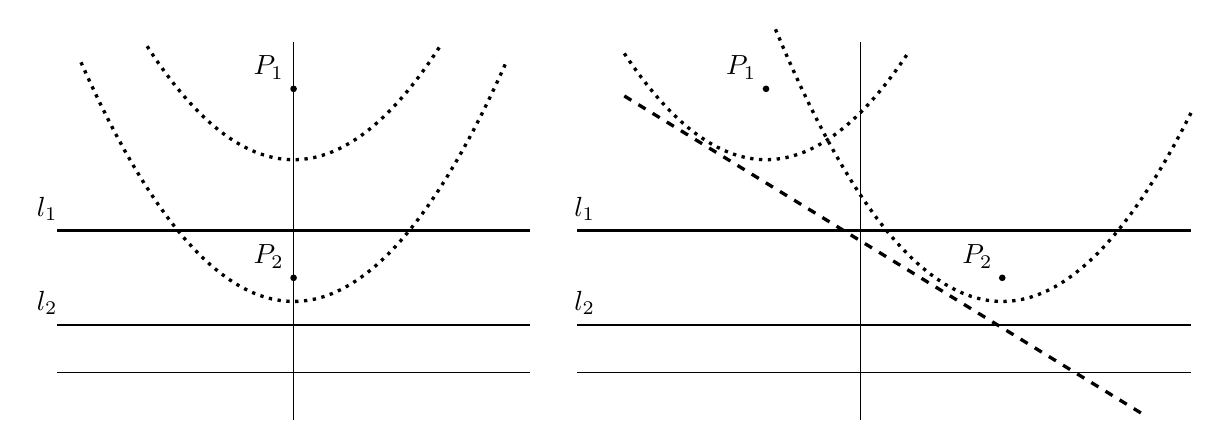
\begin{tikzpicture}[scale=.6]
\draw (-5,0) -- (5,0);
\draw (0,-1) -- (0,7);
\coordinate (P1) at (0,6);
\fill (P1) circle (2pt) node[above left] {$P_1$};
\coordinate (P2) at (0,2);
\fill (P2) circle (2pt) node[above left] {$P_2$};
\draw[thick] (-5,3) -- node[very near start,above,xshift=-25pt] {$l_1$} (5,3);
\draw[thick] (-5,1) -- node[very near start,above,xshift=-25pt] {$l_2$} (5,1);
\draw[domain=-3.1:3.1,samples=50,very thick,dotted] plot (\x,{.25*\x*\x+4.5});
\draw[domain=-4.5:4.5,samples=50,very thick,dotted] plot (\x,{.25*\x*\x+1.5});
\begin{scope}[xshift=12cm]
\draw (-6,0) -- (7,0);
\draw (0,-1) -- (0,7);
\coordinate (P1) at (-2,6);
\fill (P1) circle (2pt) node[above left] {$P_1$};
\coordinate (P2) at (3,2);
\fill (P2) circle (2pt) node[above left] {$P_2$};
\draw[thick] (-6,3) -- node[very near start,above,xshift=-25pt] {$l_1$} (7,3);
\draw[thick] (-6,1) -- node[very near start,above,xshift=-25pt] {$l_2$} (7,1);
\draw[domain=-5:1,samples=50,very thick,dotted] plot (\x,{.25*(\x+2)*(\x+2)+4.5});
\draw[domain=-1.8:7,samples=50,very thick,dotted] plot (\x,{.25*(\x-3)*(\x-3)+1.5});
\draw[very thick,dashed] (-5,5.85) -- (6,-.9);
\end{scope}
\end{tikzpicture}
\end{center}

\bigskip
\bigskip
\bigskip

%\begin{center}
%
%\begin{tikzpicture}[scale=.6]
%\draw (-7,0) -- (7,0);
%\draw (0,-1) -- (0,7);
%\coordinate (P1) at (-2,6);
%\fill (P1) circle (2pt) node[above left] {$P_1$};
%\coordinate (P2) at (3,2);
%\fill (P2) circle (2pt) node[above left] {$P_2$};
%\draw[thick] (-7,3) -- node[very near start,above,xshift=-25pt] {$l_1$} (7,3);
%\draw[thick] (-7,1) -- node[very near start,above,xshift=-25pt] {$l_2$} (7,1);
%\draw[domain=-5:1,samples=50,very thick,dotted] plot (\x,{.25*(\x+2)*(\x+2)+4.5});
%\draw[domain=-1.8:7,samples=50,very thick,dotted] plot (\x,{.25*(\x-3)*(\x-3)+1.5});
%\draw[very thick,dashed] (-5,5.85) -- (6,-.9);
%\end{tikzpicture}
%\end{center}
%
%\bigskip\bigskip
%

\begin{center}
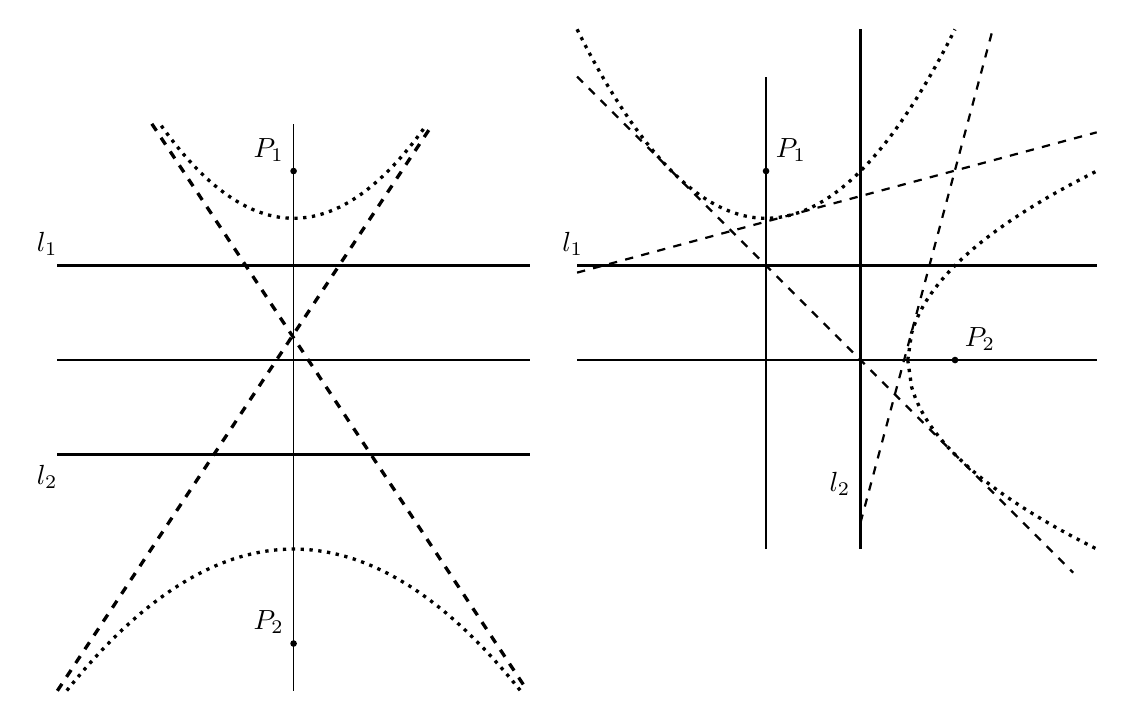
\begin{tikzpicture}[scale=.6]
\draw (-5,0) -- (5,0);
\draw (0,-7) -- (0,5);
\coordinate (P1) at (0,4);
\fill (P1) circle (2pt) node[above left] {$P_1$};
\coordinate (P2) at (0,-6);
\fill (P2) circle (2pt) node[above left] {$P_2$};
\draw[thick] (-5,2) -- node[very near start,above,xshift=-25pt] {$l_1$} (5,2);
\draw[thick] (-5,-2) -- node[very near start,below,xshift=-25pt] {$l_2$} (5,-2);
\draw[domain=-4.8:4.8,samples=50,very thick,dotted] plot (\x,{-.13*\x*\x-4});
\draw[domain=-2.8:2.8,samples=50,very thick,dotted] plot (\x,{.25*\x*\x+3});
\draw[very thick,dashed] (-5,-7) -- (2.95,5);
\draw[very thick,dashed] (-3,5) -- (4.95,-7);
\begin{scope}[xshift=10cm]
\draw (-4,0) -- (7,0);
\draw (0,-4) -- (0,6);
\coordinate (P1) at (0,4);
\fill (P1) circle (2pt) node[above right] {$P_1$};
\coordinate (P2) at (4,0);
\fill (P2) circle (2pt) node[above right] {$P_2$};
\draw[thick] (-4,2) -- node[very near start,above,xshift=-25pt] {$l_1$} (7,2);
\draw[thick] (2,-4) -- node[very near start,left] {$l_2$} (2,7);
\draw[domain=-4:4,samples=50,very thick,dotted] plot (\x,{.25*\x*\x+3});
\draw[domain=3:7,samples=50,very thick,dotted] plot (\x,{sqrt(4*\x-12)});
\draw[domain=3:7,samples=50,very thick,dotted] plot (\x,{-sqrt(4*\x-12)});

\draw[thick,dashed,domain=-4:6.5] plot (\x,-\x+2);
\draw[thick,dashed,domain=-4:7] plot (\x,.27*\x+2.93);
\draw[thick,dashed,domain=2:4.8] plot (\x,3.73*\x-10.9);
\end{scope}
\end{tikzpicture}
\end{center}

%\begin{center}
%\begin{tikzpicture}[scale=.6]
%\draw (-4,0) -- (7,0);
%\draw (0,-4) -- (0,6);
%\coordinate (P1) at (0,4);
%\fill (P1) circle (2pt) node[above right] {$P_1$};
%\coordinate (P2) at (4,0);
%\fill (P2) circle (2pt) node[above right] {$P_2$};
%\draw[thick] (-4,2) -- node[very near start,above,xshift=-25pt] {$l_1$} (7,2);
%\draw[thick] (2,-4) -- node[very near start,left] {$l_2$} (2,7);
%\draw[domain=-4:4,samples=50,very thick,dotted] plot (\x,{.25*\x*\x+3});
%\draw[domain=3:7,samples=50,very thick,dotted] plot (\x,{sqrt(4*\x-12)});
%\draw[domain=3:7,samples=50,very thick,dotted] plot (\x,{-sqrt(4*\x-12)});
%
%\draw[thick,dashed,domain=-4:6.5] plot (\x,-\x+2);
%\draw[thick,dashed,domain=-4:7] plot (\x,.27*\x+2.93);
%\draw[thick,dashed,domain=2:4.8] plot (\x,3.73*\x-10.9);
%\end{tikzpicture}
%\end{center}
